\documentclass[psfig,preprint]{aastex}
                                                                                
\begin{document}
                                                                                
\title{SOME CHARACTERISTICS OF ALFA's FIXED PATTERN NOISE (FPN)}

\author{Carl Heiles (\today)}

\tableofcontents

\clearpage

\section{INTRODUCTION}

	Accuracy of the spectra taken with ALFA and LBW are limited by
systematic baseline wiggles that change slowly, or perhaps not at all,
with time.  After a few second of integration, this {\it fixed pattern
noise}, or {\it FPN}, dominates the uncertainty in the spectrum.  It
tends to have frequency structure of width $\gtrsim 1$ MHz, which is
comparable to time delays of $\lesssim 1$ $\mu$sec in the
autocorrelation function.  We have strongly believed, and prove it here,
that the structure results from reflections, the path differences are
$\lesssim 300$ m.  1 MHz corresponds to 200 km/s at the HI line---a
velocity scale in which lots of interesting things happen,
scientifically speaking, so this FPN signifantly affects the science. 
We performed some experiments to determine some of its characteristics,
of which we report in this document. 

\section{SUMMARY OF IMPORTANT FINDINGS}

	In this section we briefly summarize our most interesting
findings. We document each in later sections with data and more
discussion. \begin{enumerate}

	\item The FPN arises from reflections and is $100\%$ polarized.
(\S \ref{100pol}, \ref{turret}, \ref{interchange})

	\item Most of the FPN arises from reflections involving shorter
path lengths.  The spectrum of delays is essentially continuous and
looks random.  (\S \ref{platform}; figures \ref{platformft11},
\ref{platformft9}, \ref{zamm_ft0}, \ref{zamm_ft6}, \ref{azmm_ft}) 

	\item A small component of the FPN arises from reflections
between the bowl and the feed and associated structures; this component
depends on the feed and the ALFA turret angle.  This component of the
FPN has sharp time-delay features in the 0.90, 1.04, and 1.16 $\mu$s. 
There seem to be additional time delays but the results look suspicious
and should be repeated.  (\S \ref{platform}; figures \ref{platformft11},
\ref{platformft9})

	\item The FPN changes when the ALFA turret is rotated. The
further the rotation, the larger the change. (\S \ref{beam})

	\item The FPN changes with zenith angle $za$. The further the
move, the larger the change. (\S \ref{za})

	\item Over the limited range in azimuth ($az$) that we tested,
the FPN changes: the further the move, the larger the change. (\S \ref{az})

	\item The FPN amplitude increases noticeably towards lower
frequencies.  (\S \ref{freq})


\end{enumerate} 
	
\section{EXPLANATION OF THE PLOTS IN FIGURES \ref{rcvr01},
\ref{rcvr1011}, and \ref{feed05}} \label{figexp1}

\begin{figure}[!p]
\begin{center}
\includegraphics[width=6in, height=4in]{rcvrplot0.ps}   
\includegraphics[width=6in, height=4in]{rcvrplot1.ps}   
\end{center}
\caption{Spectra for receivers 0 (top), 1 (bottom) on beam 0. Labels on the right
indicate ALFA turret angle; ``P'' indicates that the platform was
lowered $\sim 3$ inches. \label{rcvr01}}
\end{figure}

\begin{figure}[!p]
\begin{center}
\includegraphics[width=6in, height=4in]{rcvrplot10.ps}   
\includegraphics[width=6in, height=4in]{rcvrplot11.ps}   
\end{center}
\caption{Spectra for receivers 10 (top), 11 (bottom) on beam 5. Labels on the right
indicate ALFA turret angle; ``P'' indicates that the platform was
lowered $\sim 3$ inches. \label{rcvr1011}}
\end{figure}

\begin{figure}[!p]
\begin{center}
\includegraphics[width=6in, height=4in]{beamplot0.ps}   
\includegraphics[width=6in, height=4in]{beamplot5.ps}   
\end{center}
\caption{Spectra for beams 0 (top) and 5 (bottom). Labels on the right
indicate ALFA turret angle; ``P'' indicates that the platform was
lowered $\sim 3$ inches. \label{feed05}}
\end{figure}

	The formats of these three figures are identical.  Each figure
shows a pair of spectral plots in two panels to save space.  The spectra
are polynomial-flattened RF powers obtained from the Least-Squares
Frequency Switching (LSFS, a.k.a.\ SMARTF) procedure.  They are shown
versus r.f.\ frequency and the area near the 21-cm line (1420.4 MHz) has
been zeroed.  Each panel shows 12 plots for a specific receiver or feed;
the zeros are offset by 0.5 K for clarity and the tags on the right,
outside the plot boundary, indicate the conditions for that plot.  Each
plot shows a specific condition and time ordering of the measurements
increases from bottom to top, with about 60 seconds integration for each
plot. 

	The tags on the right show two quantities.  For each spectrum,
the first is the rms of that spectrum in milliK.  The second indicates
the ALFA turret angle, which steps in geometric increments from $0
^\circ$ to $+60 ^\circ$, then to $-60 ^\circ$, and then back to $0
^\circ$.  Near the top, the two plots labeled with a ``P'' indicate that
the platform was lowered by $\sim 3$ inches.  The first plot, at the bottom, is
the spectrum for the first measurement of the series of 13; it has ALFA
turret angle $0 ^\circ$.  All the other plots are {\it differences}
between its particular spectrum and the first spectrum.  This is why the
very top plot, which was also taken at ALFA turret angle $0 ^\circ$ (but
about 30 minutes later), is so small. 

\section{BEAM 0 SHOWS THAT THE FPN IS 100\% POLARIZED} \label{100pol}

	First let's take a look at the on-axis feed 0, which is served
by receivers 0 and 1.  This feed is almost on-axis, so when we rotate
the ALFA turret all that happens is the feed rotates with only a little
translation---in other words, the polarization position angle changes. 
Look at Figure \ref{rcvr01}, which shows the difference between
receivers 0 and 1 for different position angles.  As we move away from
ALFA angle 0, the difference spectra rms's get larger.  This reflects
the polarization of the FPN, and shows that the FPN is polarized. 

	The fluctuations in the two receivers, which have orthogonal
linear polarizations, are completely uncorrelated.  For the ALFA turret
angle $0 ^\circ$ spectrum, the rms of the difference between the two
receivers' spectra is 163 milliK and that of the sum is 164 milliK,
which is close enough to equality to consider the spectral fluctuations
in the two receivers to be completely uncorrelated and independent.  If
the FPN were randomly polarized, then the FPN wouldn't change at all with
position angle; the rms of the difference between the two receivers
would be zero.  The fact that the rms's of the difference and sum are
identical means that the FPN is $100\%$ polarized. 

	For off-axis feeds we can make the equivalent of Figure
\ref{rcvr01}; for feed 5 we show the plots for its receivers 10 and 11
in Figure \ref{rcvr1011}. We show this for fun only because it doesn't
mean much: the native linear polarizations in all feeds are oriented
identically on the sky, so as we rotate the ALFA angle we also rotate
the orientation of the linear polarizations to which a feed responds.
Because the FPN is itself polarized, the response of individual
receivers contains this changing polarization. Instead of looking at
individual receivers for a feed, we have to look at their sum so that
the polarization of the FPN doesn't confuse us.

\section{DEPENDENCE OF FPN ON ALFA TURRET ANGLE} \label{turret}

	Figure \ref{feed05} shows the spectra for the on-axis feed 0
(top panel) and the off-axis feed 5 (bottom panel).  Note that these are
averages of both receivers, so FPN polarization plays no role in these
plots.  As we increase the ALFA turret angle away from $0^\circ$, the
FPN of the difference spectra rise.  (These are difference spectra, each
spectrum minus the one for turret angle 0).  The rms for feed 0 rises
modestly, by no more than a factor of 2.  This as it should be: when we
rotate the ALFA turret, all we are doing is rotating feed 0, so when we
add the polarizations we expect zero effect.  The residual effect that
we do see is almost certainly produced by feed 0 being slightly off-axis
(by design; Cort\'ez-Medellin 2002). 

	For the outrigger feeds the FPN changes quite rapidly with
turret angle.  For example, for turret angle $8^\circ$, for beam 5 the
rms of the difference spectrum is almost half the value of the
turret-angle 0 spectrum.  Thus, even at $8^\circ$ turret angle, the FPN
has changed a lot from its pattern at $0^\circ$. 

\section{DEPENDENCE OF FPN ON FEED} \label{beam}

\begin{figure}[!p]
\begin{center}
\includegraphics[width=6in]{quickfig.ps}   
\end{center}
\caption{An example of spectra for each of the receivers. The mean of all
receivers is at the top. Each receiver's spectrum is stastically
independent of the others'. \label{quickfig}}
\end{figure}

	The FPN of each feed is statistically independent of the others. 
Figure \ref{quickfig} shows one set of spectra all 14 receivers,
together with the mean at the top.  The FPN for the mean is much smaller
than the FPN of the individual receivers.  In fact, a detailed look at a
set of data (not those in the figure) shows that the statistical
reduction in the rms of the mean spectrum is almost exaclty what's
expected if the FPN's are statistically independent.  Thus, the rms of
the FPN of the average of all receivers is about $\sqrt{14}$ times smaller
than the average rms of each, which is what we expect for statistical
independence. 

	There is no comprehensible systematics in variation of the FPN
rms from beam to beam.  A grand average over {\it all} of the 12
measurement conditions gives, for the 7 beams, rms's of [83, 62, 79, 83,
81, 84, 78] milliK.  This average mixes all of the ALFA turret angles
that we sampled.  If we restrict the average to turret angle 0, we
obtain [81, 66, 82, 89, 78, 93, 86] milliK.  For both cases, feed 1 is
significantly smaller than the others; the others are comparable to each
other.  Feeds 1 and 6 are the ``downhill'' feeds, closest to the center
of the Gregorian dome.  Feeds 3 and 4 are the ``uphill'' feeds.  But it
doesn't seem to matter. 

\section{THE FPN STAYS FIXED IN SPACE WHEN WE ROTATE ALFA BY 60 DEGREES}
\label{interchange}

	If the FPN is from reflections, then it should be fixed in
space.  When we rotate the ALFA turret by $60^\circ$, thus interchanging
one feed for another, the newly-interchanged feed should see the same
FPN that the original one did.  This is, in fact, the case.  However,
the FPN interchanges are not quite perfect

\begin{figure}[!p]
\begin{center}
\includegraphics[width=6in]{ccfplot.ps}   
%\includegraphics[width=6in, height=4in]{rcvrplot1.ps}   
\end{center}
\caption{Difference spectra for ALFA turret angles $-60^\circ$, $0^\circ$, and
$60^\circ$. In each panel, the top spectrum is the ``self difference''
and the bottom one the ``interchange difference''. The latter is the
spectrum of the interchanged receiver minus that of the original. See
text! \label{ccfplot}}
\end{figure}

\begin{figure}[!p]
\begin{center}
\includegraphics[width=6in]{ccfplot_ft.ps}   
%\includegraphics[width=6in, height=4in]{rcvrplot1.ps}   
\end{center}
\caption{ACF's of interchange difference spectra for ALFA turret 
angles $-60^\circ$, $0^\circ$, and
$60^\circ$\label{ccfplot_ft}}
\end{figure}

	First, let us define the terms {\it self difference} and {\it
interchange difference}. These differences are between receivers at two
different turret angles that differ by $60^\circ$ or $120^\circ$. The
self difference is between the same feed at the two angles. The
interchange difference is the difference between the original feed and
the one that occupied the same physical location after the rotation. 

	We show three representive cases in Figure \ref{ccfplot}.  The
top panel compares turret angles $[-60^\circ, 0^\circ]$; the middle,
$[+60^\circ, 0^\circ]$; and the bottom, $[60^\circ,-60^\circ]$.  We
subtract feed 5's spectrum at the first angle from its spectrum at the
second angle (upper plot in each panel); and from the spectrum of its
interchange partner (lower plot). 

	For each panel, the interchange difference (lower plot) looks
much less noisy than the self difference.  This proves that the FPN stays
fixed in space and as the feeds rotate they sample the same reflections
in space.  However, the interchange difference isn't just thermal noise,
so there is more to the story.  The ACF plots figure \ref{ccfplot_ft} show that
the differences are primarily associated with short time delays. In
particular, for the lower two plots the ACF shows a well-defined peak at
a delay of 0.075 $\mu$s (22.5 meters round trip, 11.25 meters one-way),
and you can clearly see the associated low-frequency ripple on the
right-hand half of the frequency spectrum. 

	Either there is an additional contributor to FPN that is
receiver-based, or there are mechanical imperfections or anomalies.  We
don't think the receivers themselves have any intrinsic FPN because of
tests we did in July 2005, when we observed with the ALFA cover on and
found {\it no} FPN.  The 11.25 meter one-way distance perhaps offers a
hint about what might be happening to someone who knows the mechanical
structural details. 

\section{BEHAVIOR OF THE FPN WITH PLATFORM HEIGHT}
\label{platform}

	A well known reflection is that between the bottom of the bowl
and the feed, Gregorian, or platform.  If we change the platform height
while keeping all other conditions the same, we change the phase of
these reflections and we can see what happens.  Here we look at two
feeds, the on-axis feed 0 and feed 5 as a representative; all of the
off-axis feeds looked similar.  We have two platform-moved datasets, one
at ALFA turret angle $-60^\circ$ and one at angle $0^\circ$; the mighty
Phil grabbed hold of the platform, moved its great weight of the
platform down by $\sim 3$ inches\footnote{The tiedowns moved 5 inches.}
and held it there for a few minutes to make our measurements, and then
lifted it back up. 

\subsection{Plots of spectra---Kelvins versus frequency}
\begin{figure}[!p]
\begin{center}
\includegraphics[width=6in]{platform11.ps}   
\end{center}
\caption{Difference spectra for ALFA turret angle $0^\circ$. 
The top panel is feed 0 and the bottom feed 5. In each panel,
the top spectrum is the difference spectrum for the two platform heights
and the bottom spectrum is one of the spectra. \label{platform11}}
\end{figure}

\begin{figure}[!p]
\begin{center}
\includegraphics[width=6in]{platform9.ps}   
\end{center}
\caption{Difference spectra for ALFA turret angle $-60^\circ$. 
The top panel is feed 0 and the bottom feed 5. In each panel,
the top spectrum is the difference spectrum for the two platform heights
and the bottom spectrum is one of the spectra. \label{platform9}}
\end{figure}

	Figure \ref{platform11} shows the dependence on platform height
for ALFA turret angle 0. This is what we'd expect: nearly everything
should cancel out in the upper difference plots, and what remains
should be a rapid ripple with period $\sim 1$ MHz, which reflects the
$\sim 1$ $\mu$sec delay time of the feed-to-bowl reflection. Both the
on-axis and off-axis beams have roughly the same behavior.

	Figure \ref{platform9} is a completely different story. Feed 0
shows the same, expected, behavior as in Figure \ref{platform11}. But
look at feed 5---it's completely different! The difference spectrum
doesn't cancel out at all. Rather, it looks similar in shape to the
actual spectrum! {\it All} of the off-axis feeds show this same effect!

\subsection{Plots of autocorrelation functions---Kelvins versus time delay}

	Figures \ref{platformft11} and \ref{platformft9} are the
autocorrelation function (acf) equivalents of figures \ref{platform11} and
\ref{platform9}.  The acf is the Fourier transform of the power
spectrum and vice-versa. A peak in the acf indicates a reflection with a
corresponding round-trip time delay. The distance for 1 $\mu$sec is
about 1000 ft, which is about twice the distance between the feed and
the bottom of the bowl. 

\begin{figure}[!p]
\begin{center}
\includegraphics[width=6in]{platform_ft11.ps}   
\end{center}
\caption{ACF's for ALFA turret angle $0^\circ$. 
The top panel is feed 0 and the bottom feed 5. In each panel,
the top acf is the difference between acf's for the two platform heights
and the bottom acf is one of those acf's. Time delay in $\mu$sec;
KELVINS is the amplitude of the Fourier component. \label{platformft11}}
\end{figure}

\begin{figure}[!p]
\begin{center}
\includegraphics[width=6in]{platform_ft9.ps}   
\end{center}
\caption{ACF's for ALFA turret angle $-60^\circ$. 
The top panel is feed 0 and the bottom feed 5. In each panel,
the top acf is the difference between acf's for the two platform heights
and the bottom acf is one of those acf's. Time delay in $\mu$sec;
KELVINS is the amplitude of the Fourier component. \label{platformft9}}
\end{figure}

	Figure \ref{platformft11} shows the acf's for feed 0 (top panel)
and feed 5 (bottom panel) for ALFA turret angle 0.  The behavior is
somewhat curious.  For beam 5, the difference acf has a single sharp
spike at 0.91 $\mu$sec.  For beam 0, the difference has a
dominant peak at $0.91$ $\mu$sec but it's rattier, with
substantial peaks at 1.04 and 1.16 $\mu$sec, as well as a broader
underlying shelf running from about 0.7 to 1.4 $\mu$sec.  (We
conservatively estimate the accuracy of all quoted times to be $\pm
0.005$ $\mu$sec; the time resolution is 0.01 $\mu$sec). 

	Figure \ref{platformft9} shows the acf for feed 0 (top panel)
and feed 5 ( bottom panel) for ALFA turret angle $-60^\circ$.  The
behavior is a lot weirder than in Figure \ref{platformft11} for angle
$0^\circ$.  Here, for the difference acf for feed 5, instead of the nice
single sharp peak in figure \ref{platformft11} we have a very broad
response that covers roughly the same time delays as the acf's
themselves.  The two peaks near 0.9 $\mu$s are barely recognizable; they
have delays 0.90 and 0.94 $\mu$s.  The 0.90 $\mu$sec peak differs from
the prominent turret angle 0 peak by 0.01 $\mu$s, equivalent to a total path of
$\sim 10$ feet.  This ratty behavior for feed 5 is, of course, exactly
what we expect from looking at the frequency spectra in Figure
\ref{platform9}.  For beam 0, we have the same three dominant spikes as
before at 0.91, 1.04, and 1.16 $\mu$sec, together with the broad
underlying shelf, but there is also substantial power below $\sim 0.4$
$\mu$s. 

	It's hard to understand why there should be such a difference
between turret angles $-60^\circ$ and $0^\circ$.  It is worth trying
this experiment again.  These experiments were done during the daytime,
and perhaps a Solar reflection interfered with the data for ALFA turret
angle $-60^\circ$.  On the other hand, the large power for the platform
difference spectra for feed 5 occurs for all the off-axis feeds as
well, and why should their behavior differ from that of feed 0? Who
knows. 

\section{ZA DEPENDENCE OF FPN} \label{za}

\begin{figure}[!p]
\begin{center}
\includegraphics[width=6in, height=4in]{zmmplot0.ps}   
\includegraphics[width=6in, height=4in]{zmmplot5.ps}   
\end{center}
\caption{ZA dependence of FPN for feeds 0 (top) and 5 (bottom). All
spectra except the middle one are difference spectra, equal to that
spectrum minus the middle one. Labels on the right
indicate: first the rms in milliK, and second the mean $za$ for the spectrum.
\label{zmm05}}
\end{figure}

	Here we examine the $za$ dependence of the FPN.  Figure
\ref{zmm05} shows the FPM for 7 different intervals of $za$ ranging from
$3.0^\circ$ to $19.7^\circ$.  The FPN changes slowly with %za$; the
change from one extreme to the other is comparable to the FPN itself. 
All feeds have about the same behavior. 

\begin{figure}[!p]
\begin{center}
\includegraphics[width=6in]{zammplot_ft0.ps}   
\end{center}
\caption{Difference acf's for all feeds at $\langle za
\rangle=4.0^\circ$, where the FPN is large (Figure \ref{zmm05}).  Feed
number increases upwards.  The difference acf is the Fourier transform
of the spectrum minus the spectrum at $za = 12.5^\circ$.  Feed number
increases upwards.  \label{zamm_ft0}}
\end{figure}

\begin{figure}[!p]
\begin{center}
\includegraphics[width=6in]{zammplot_ft6.ps}   
\end{center}
\caption{Difference acf's for all feeds at $\langle za
\rangle=19.7^\circ$, where the FPN is large (Figure \ref{zmm05}).  Feed
number increases upwards.  The difference acf is the Fourier transform
of the spectrum minus the spectrum at $za = 12.5^\circ$.  Feed number
increases upwards.  \label{zamm_ft6}}
\end{figure}

	Figures \ref{zamm_ft0} and \ref{zamm_ft6} show, for all feeds,
the acf's of the difference between the spectra at $\langle za
\rangle=[4.0^\circ, 19.7^\circ]$ and those at $\langle za \rangle =
12.5^\circ$.  Most of the energy resides below delays of a $\mu$s, and
there are few prominent peaks.  In Figure \ref{zamm_ft0}, the prominent
peaks for feed 0 are at 0.91 and 1.04 $\mu$s; the prominent peak for
feed 6 is at 0.90 $\mu$s.  In Figure \ref{zamm_ft6}, the prominent peak
in several spectra is at 1.04 $\mu$s; the prominent peak for feed 3 is
at 0.79 $\mu$s. 

\section{AZ DEPENDENCE OF FPN} \label{az}

\begin{figure}[!p]
\begin{center}
\includegraphics[width=6in, height=4in]{azmmplot0.ps}   
\includegraphics[width=6in, height=4in]{azmmplot5.ps}   
\end{center}
\caption{AZ dependence of FPN for feeds 0 (top) and 5 (bottom). Labels on the right
indicate: first the rms in milliK, and second the mean $az$ for the spectrum.
All spectra except the third from the bottom (the reference spectrum); 
difference spectra, being the spectrum itself minus the reference spectrum.
\label{azmm05}}
\end{figure}

\begin{figure}[!p]
\begin{center}
\includegraphics[width=6in]{azmmplot_ft.ps}   
\end{center}
\caption{ACF of the $az$ difference spectra for all
feeds at $az=189^\circ$ (Fourier transforms of the topmost spectra in
Figure \ref{azmm05}). For all feeds, the prominent peaks occur at
0.79, 0.90, 0.98, and 1.04 $\mu$s. 
\label{azmm_ft}}
\end{figure}

	Here we examine the $az$ dependence of the FPN.  Figure
\ref{azmm05} shows the FPM for 7 different intervals of $az$ ranging
from $269^\circ$ to $189^\circ$ in increments of $\sim -20^\circ$.  The
columns of numbers on the right hand side of the plots indicate, first,
the rms of the spectrum; and second, the mean $az$.  All of these except
the third from the bottom (which is the reference spectrum) are
difference spectra, equal to the spectrum itself minus the reference
spectrum.  All of these data are at $za=18^\circ$ except the bottom one,
which is at $za \sim 19.5^\circ$; this $za$ difference probably
explains the larger difference spectrum. 

	If everything were perfect, the FPN would not change with $az$. 
In fact, as $az$ changes the spectra do indeed change slowly; you need
to go $\sim 40^\circ$ before the differences become comparable to the
FPN itself.  We examined the rms's for all feeds and found that the
uphill feeds 3 and 4 have a $\sim 30\%$ larger rms for the top spectrum
than the other feeds.  This probably occurs because these feeds see a
bit more of the ground than the other feeds.  If so, these small
feed-to-feed differences with $az$ should disappear at smaller $za$. 

	Figure \ref{azmm_ft} shows the acf's for the topmost spectra in
Figure \ref{azmm05}, for all 7 feeds.  The prominent
peaks occur at 0.79, 0.90, 0.98, and 1.04 $\mu$s; some peaks appear in some
feeds and not others. Feed 0, the on-axis feed, has the most prominent
peaks.

\section{FREQUENCY DEPENDENCE OF FPN} \label{freq}

	Look at all of the preceding plots: the amplitude of the FPN
increases towards lower frequencies.  This suggests that the reflections
are not purely specular, but at least partly diffractive, and that they
are produced by structures whose sizes are comparable to the wavelengths
involved---maybe the structural beams on the platform. 

	This frequency dependence has important ramifications for the
representation of the FPN by Fourier modes. The Fourier representation
is a natural one for reflections because of the acf/power spectrum
relationship. However, the frequency variation of the FPN indicates that
the strength of the reflections varies across our 100 MHz band, which
implies that the Fourier coefficients decrease in amplitude with
increasing frequency---contrary to the basic assumption in Fourier
transforms that the coefficients apply all across the interval being
analyzed. This suggests that a modification of the Fourier
representation is required. Hmmmmmmmmmmm\dots

\acknowledgements

	This research was supported in part by NSF grant AST 04-06987
and by the NAIC.  It is a pleasure to thank Phil Perillat for his
invaluable interest, assistance, and expertise. 

\begin{references}
\reference {} Cort\'ez-Meddelin, G. 2002, Arecibo Focal Array Memo
Series, ``Final Feed Selection Study for the Multi Beam Array System''.

\end{references}
\end{document}
		
